%\section{Searching for better DLMalloc parameters}
\section{Deep Parameter Optimisation}

Our approach takes three steps. Firstly we apply Mutation Operators to generate variants of the original \emph{dlmalloc} in order to understand which pieces of the source code could be more influential to the performance. Secondly we analyze the sensitivity of each mutated piece by evaluating the variants on a given set of applications and testsuites. After locating the most interesting and influential part of the code, we expose them to users so that they could be modified from the outside as needed. Thirdly, we apply SBSE approach to find the optimal values for both the existing and exposed parameters for each of the given applications.This section first discusses how we find and expose interesting parameters.

%** maybe need add some think to justiy the choice of self-implementation. 

\begin{figure}[htbp]
\centering
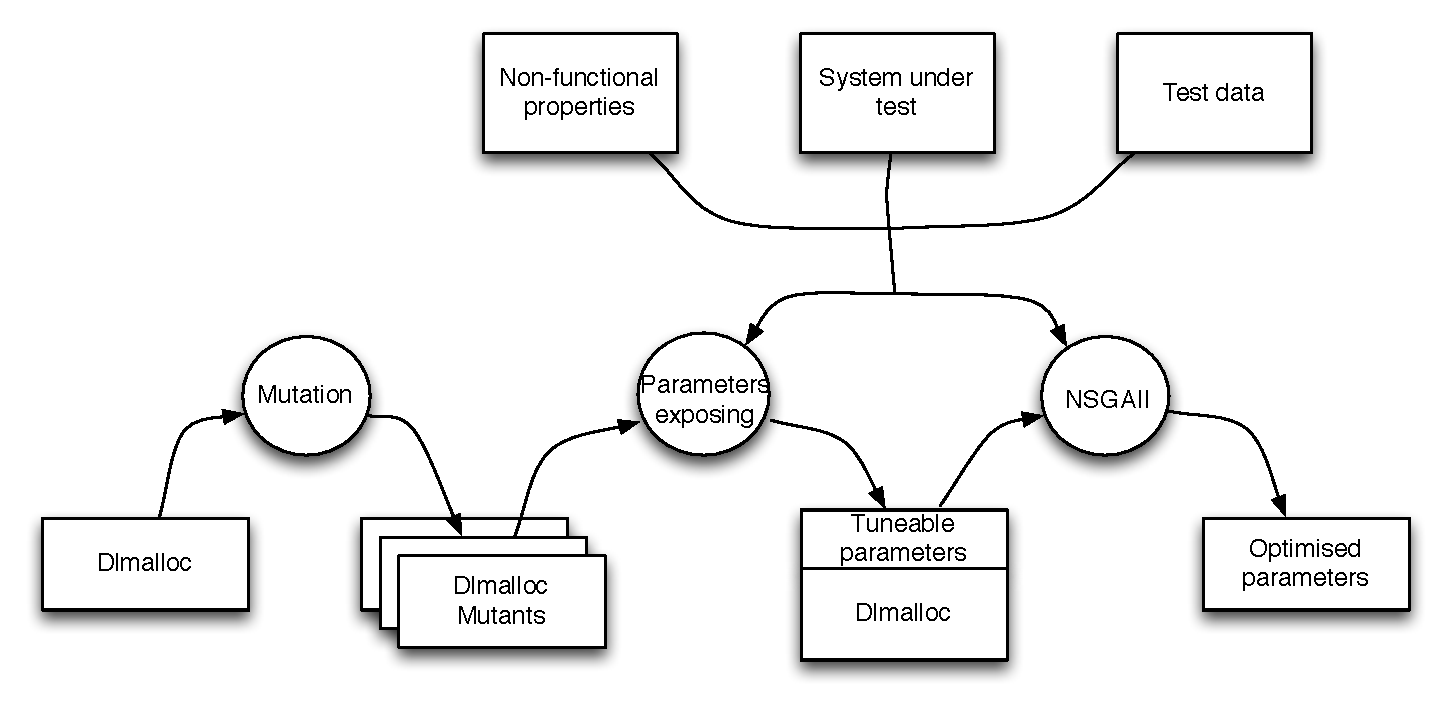
\includegraphics[width=3.2in]{pics/system}
\caption{Deep parameter optimisation workflow}\label{system}
\end{figure}


\subsection{Exposing Implicit Parameters}
Other than the existing parameters introduced above, there might be some other valuable variables which could influence the performance of the allocator but burried and neglected in the massive source code. It could be a constant, an expression or even a predicate. In this paper we try to expose these valuable parts of \emph{dlmalloc} to users so that they can also adjust these parts to fit their needs. Other than blindly exposing random parameters, we need to know how much each piece of code could influence the behavior of \emph{dlmalloc} before we expose it. In another word, we need sensitivity analysis.

% Introduce two types of mutations and why
In order to obtain the sensitivity information, one simple way is to delete each statement at a time to see how important this statement is to the performance of \emph{dlmalloc}. However, when the statement deleted is consist of a very complicated expression, which variable or operator is more important than others remains unknown. 

A more advanced way to obtain the sensitivity information is via Mutation Operators. Mutation Operators are used in Mutation Testing, which automatically inserts some faults to a target program via Mutation Operators to generate mutants of this program and try to detect those faults using a test suite to see whether the test suite is good enough to reveal program faults. 

In this work, we just use these Mutation Operators to slightly alter \emph{dlmalloc}, in order to understand which piece of source code influences the memory consumption most. We apply both the statement deletion way and Mutation Operator way in the sensitivity analysis and compare their effectiveness, which is reported later. In either way, there are many variants of original \emph{dlmalloc} generated, all of them only differ from the original in at most one statement. We then evaluate and record the performance of these variants on the subject applications and corresponding test suites. This helps us understand the most influential pieces of code in the original \emph{dlmalloc}.

According to the sensitivity information abtained above, we pick the most influential statements and expose part of them as configurable parameters that can be modified at compilation, just like the other existing parameters introduced in section \ref{sec_dlmalloc_tunable_parameters}. These exposed parameters include constants, expressions and predicates. 

For constants, exposure is no more than replacing it with a variable that can be defined externally. For expressions and predicates things get a little more compilcated. We obtained different version of an expression or a predicate from the sensitivity information and create a selection statement to include all different versions. In this way, which version of expression or predicate is used can be controled by modifying an external numerical value that controls the selection statement.
% maybe talk about rank


\subsection{MultiObjective Paramter optimisation}
\label{sec_nsgaii}
In this work, we apply NSGA II\cite{996017}, a multi-objective Genetic Algorithm, on the searching of the optimal values for those \emph{dlmalloc} parameters list above.
% data representation
Since these parameters can be easily interpreted as integers, we use linear representation to store each candidate, in which each gene is an integer number representing one of the parameters. For mutation, we use different operators according to each gene's legitimate range, while two-point crossover is applied.
% fittness evaluation

Since we need to re-compile \emph{dlmalloc} every time we change the parameters, in order to minimize compilation cost, we only compile \emph{dlmalloc} to a shared object and each application is compiled and linked to that shared object at the beginning of each experiment. In each generation, after new candidates are generated through mutation and crossover operators, each candidate is re-compiled and run with a given subject application. When the performance of the application with each candidate version of \emph{dlmalloc} is collected, an NSGA II style selection is applied to obtain the next generation.
% how to measure time
% how to measure memory

Currently we focus on two non-functional properties: time and memory consumption. \emph{Glibc}'s \emph{wait4} function is used to calculate the cpu time consumed by the application (sum of user time and system time), while we compute the high-water mark of the memory consumption by instrumentation of \emph{dlmalloc}. In this way the memory measured is virtual memory, because the physical pages allocated to an application is not always deterministic but depends on the work load and the system so that measuring the physical memory usage could be hard and misleading.
